\documentclass[a4paper,10pt]{article}
\usepackage[utf8]{inputenc}
\usepackage[margin=1in]{geometry}
\usepackage{amsmath, amssymb, dsfont}
\usepackage{braket}
\usepackage{hyperref}
\usepackage{xcolor}
\usepackage{subfigure}
\usepackage{graphicx}
\hypersetup{
    colorlinks,
    linkcolor={blue!70!black},
    citecolor={blue!70!black},
    urlcolor={blue!70!black}
}

%opening
\title{A primer on quantum RAM}
\author{Olivia Di Matteo}

\begin{document}

\maketitle

\abstract{\textcolor{red}{\textbf{This document is a work in progress} and is being continuously edited.}{ 

\tableofcontents

\section{Introduction and FAQ}

Quantum RAM (qRAM) has gained some notoriety in the past few years, and attitudes toward it depend quite heavily on the circles you run in. The goal of this set of notes is to provide a general overview of the subject, as well as discuss some very specific implementations. It is meant to be a companion to the Q\# qRAM libraries we are writing (cite the repo), but can also serve as a standalone reference.

In my experience, explaining qRAM to someone boils down to answering a handful of key questions. I'll provide some potentially unsatisfactory answers up front, but go into far more detail in the next few sections\footnote{Those details may not be satisfactory either.}.

\begin{enumerate} 
 \item \textbf{Do I need a qRAM?}
  \emph{Sometimes}. You'll need a qRAM, or some more general means of \emph{quantum state preparation} in quantum machine learning (QML) algorithms that require you to load in classical data, or query an oracle that returns classical data. I've heard a number of stories of people working on QML being actively discouraged from doing so because ``QML won't work without a qRAM''. That's just not true, because \emph{many QML algorithms do not need a qRAM}. Now, whether or not they yield any quantum advantage is a separate question, and won't be discussed here. The key point I want to make is that \emph{some} QML algorithms need a qRAM, and they will potentially run into trouble as per the next question.
 \item \textbf{Can we design an efficient qRAM?} \emph{Maybe.} In this primer we'll take a look at proposals that will in principle run in polynomial depth, and others that scale far worse. There are some very interesting qubit-time tradeoffs one can explore, in particular if the data being stored has some sort of underlying structure. Regardless, even if we can design an efficient circuit, we'd also like something that is efficient in a fault-tolerant setting, and this is potentially very expensive.
 \item \textbf{Can I build one?} \emph{Maybe.} No one has actually done so, but there are a handful of hardware proposals that will be discussed in more detail in \autoref{sec:hardware}. 
\end{enumerate}


%%%%%%%%%%%%%%%%%%%%%%%%%%%%%%%%%%%%%%%%%%%%%%%%%%%%%%%%%%%%%%%%%%%%%%%%%%%%%%%%%%
%%%%%%%%%%%%%%%%%%%%%%%%%%%%%%%%%%%%%%%%%%%%%%%%%%%%%%%%%%%%%%%%%%%%%%%%%%%%%%%%%%
%%%%%%%%%%%%%%%%%%%%%%%%%%%%%%%%%%%%%%%%%%%%%%%%%%%%%%%%%%%%%%%%%%%%%%%%%%%%%%%%%%
%%%%%%%%%%%%%%%%%%%%%%%%%%%%%%%%%%%%%%%%%%%%%%%%%%%%%%%%%%%%%%%%%%%%%%%%%%%%%%%%%%
%%%%%%%%%%%%%%%%%%%%%%%%%%%%%%%%%%%%%%%%%%%%%%%%%%%%%%%%%%%%%%%%%%%%%%%%%%%%%%%%%%

\section{A brief history of the brief history of quantum machine learning}
\label{sec:qml}

%%%%%%%%%%%%%%%%%%%%%%%%%%%%%%%%%%%%%%%%%%%%%%%%%%%%%%%%%%%%%%%%%%%%%%%%%%%%%%%%%%
%%%%%%%%%%%%%%%%%%%%%%%%%%%%%%%%%%%%%%%%%%%%%%%%%%%%%%%%%%%%%%%%%%%%%%%%%%%%%%%%%%
%%%%%%%%%%%%%%%%%%%%%%%%%%%%%%%%%%%%%%%%%%%%%%%%%%%%%%%%%%%%%%%%%%%%%%%%%%%%%%%%%%
%%%%%%%%%%%%%%%%%%%%%%%%%%%%%%%%%%%%%%%%%%%%%%%%%%%%%%%%%%%%%%%%%%%%%%%%%%%%%%%%%%
%%%%%%%%%%%%%%%%%%%%%%%%%%%%%%%%%%%%%%%%%%%%%%%%%%%%%%%%%%%%%%%%%%%%%%%%%%%%%%%%%%

\section{Encoding classical data on a quantum computer}
\label{sec:encoding}

There is a nice overview of the encodings below in \cite{Schuld2018}.

\subsection{Basis encoding}

Give overview of the basis encoding, i.e.
\begin{equation}
 \hbox{data} \enskip 01001 \rightarrow \ket{01001}
\end{equation}


\subsection{Quantum RAM / ROM}

Query as bits in superposition:
\begin{equation}
 \sum_i \ket{i} \ket{0} \rightarrow \sum_i \ket{i} \ket{b_i}
\end{equation}

Query as phase in superposition (applications to Grover)
\begin{equation}
 \sum_i \ket{i} \rightarrow \sum_i (-1)^{b_i} \ket{i}
\end{equation}


\subsection{Quantum state preparation (amplitude encoding)}

Given some vector $\mathbf{a} = \left( a_0, \cdots,  a_{n-1} \right)$, create the quantum state
\begin{equation}
 \ket{\psi} = \sum_{i=0}^{n-1} a_i \ket{i}
\end{equation}

Discuss how this relies on having a qROM as an underlying subroutine.


%%%%%%%%%%%%%%%%%%%%%%%%%%%%%%%%%%%%%%%%%%%%%%%%%%%%%%%%%%%%%%%%%%%%%%%%%%%%%%%%%%
%%%%%%%%%%%%%%%%%%%%%%%%%%%%%%%%%%%%%%%%%%%%%%%%%%%%%%%%%%%%%%%%%%%%%%%%%%%%%%%%%%
%%%%%%%%%%%%%%%%%%%%%%%%%%%%%%%%%%%%%%%%%%%%%%%%%%%%%%%%%%%%%%%%%%%%%%%%%%%%%%%%%%
%%%%%%%%%%%%%%%%%%%%%%%%%%%%%%%%%%%%%%%%%%%%%%%%%%%%%%%%%%%%%%%%%%%%%%%%%%%%%%%%%%
%%%%%%%%%%%%%%%%%%%%%%%%%%%%%%%%%%%%%%%%%%%%%%%%%%%%%%%%%%%%%%%%%%%%%%%%%%%%%%%%%%


\section{Bucket-brigade quantum RAM}
\label{sec:bb}

\textbf{[These paragraphs are lifted from my thesis and need to be edited and expanded on].}

Architectures for qRAM began to emerge roughly a decade ago with the bucket brigade model of \cite{Giovannetti2008, Giovannetti2008b}. In this model, $2^n$ bits of classical data (that we would like to quantumly query) are stored in the $2^n$ leaves of a binary tree, as depicted in. The nodes of the tree relate to the address, with the $j$-th address bit corresponding to the $j$-th layer of the tree, as will be described below. 

\begin{figure}
 \centering
 \begin{subfigure}
    \centering
    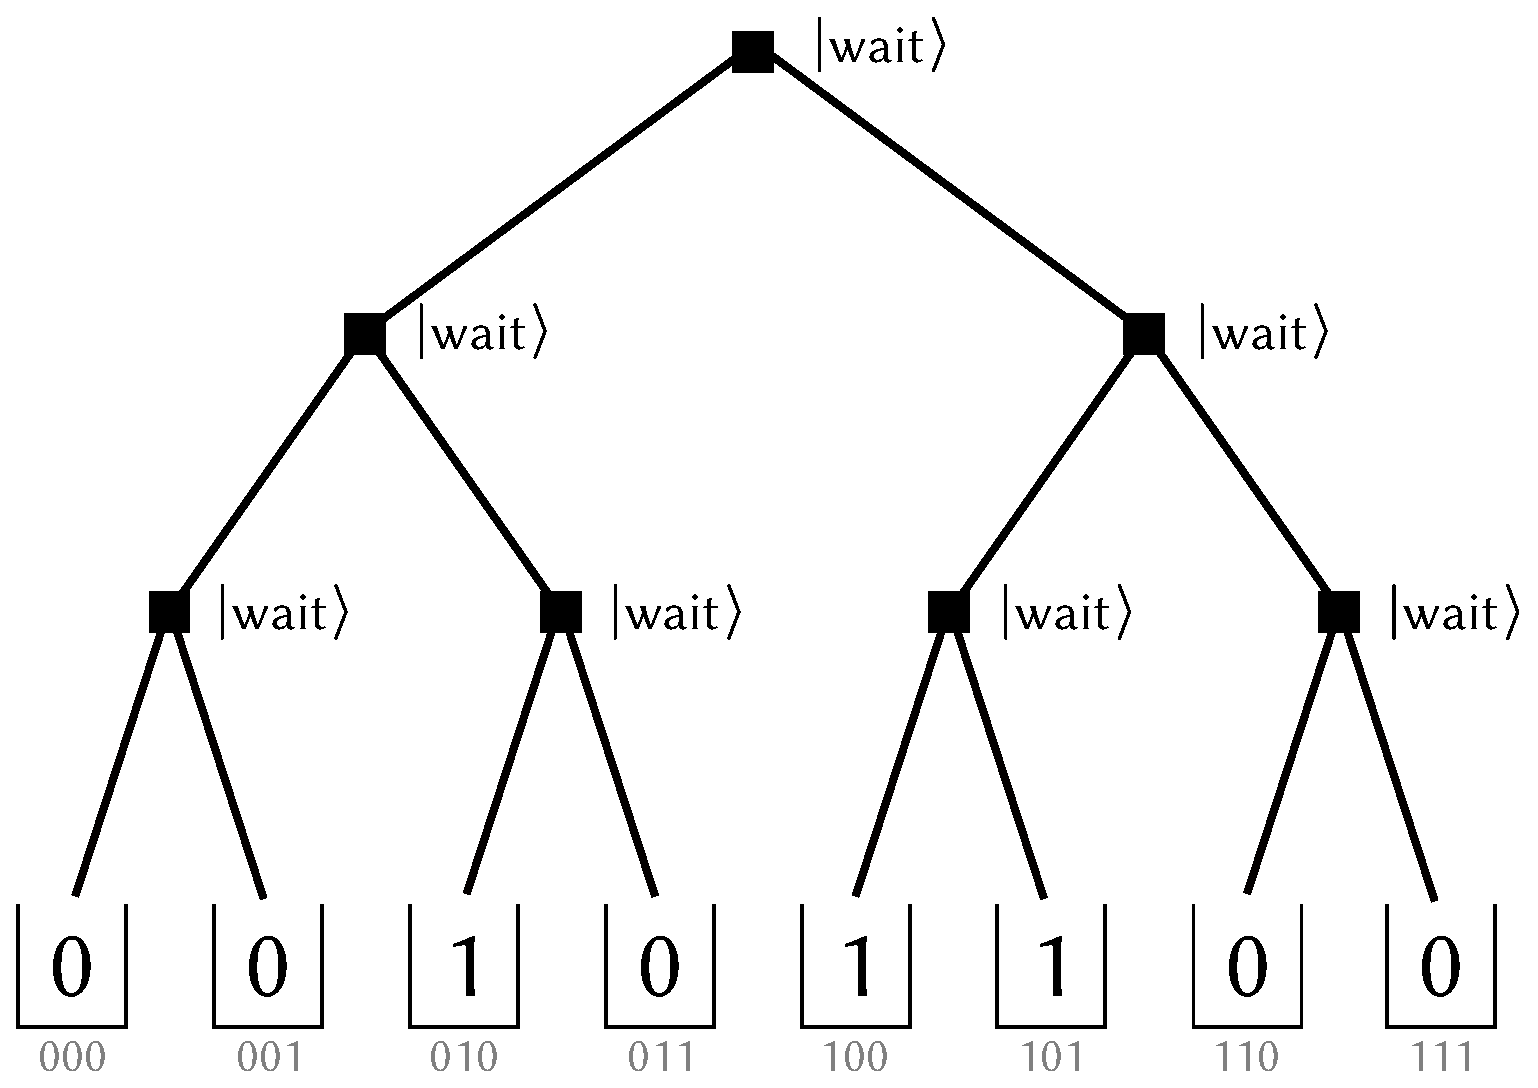
\includegraphics[height=2in]{fig/bb-00}
 \end{subfigure}
  \hspace{0.5cm}
  \begin{subfigure}
    \centering
    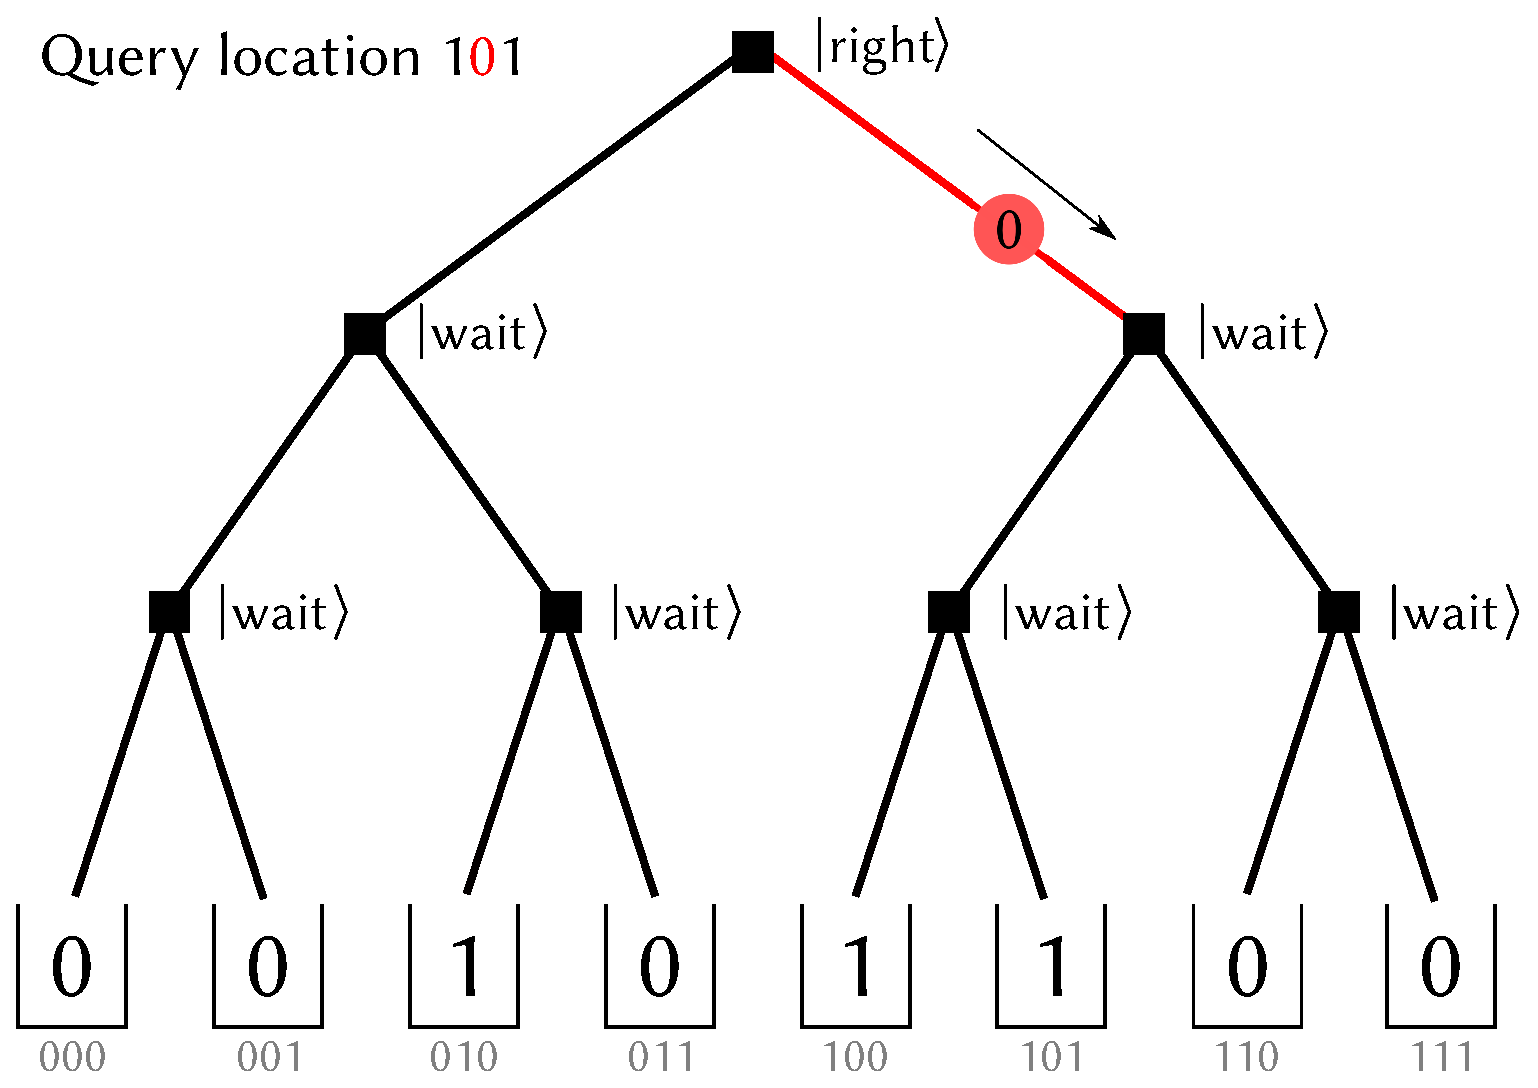
\includegraphics[height=2in]{fig/bb-01}
 \end{subfigure} \\
    \vspace{0.5cm}
     \begin{subfigure}
        \centering
        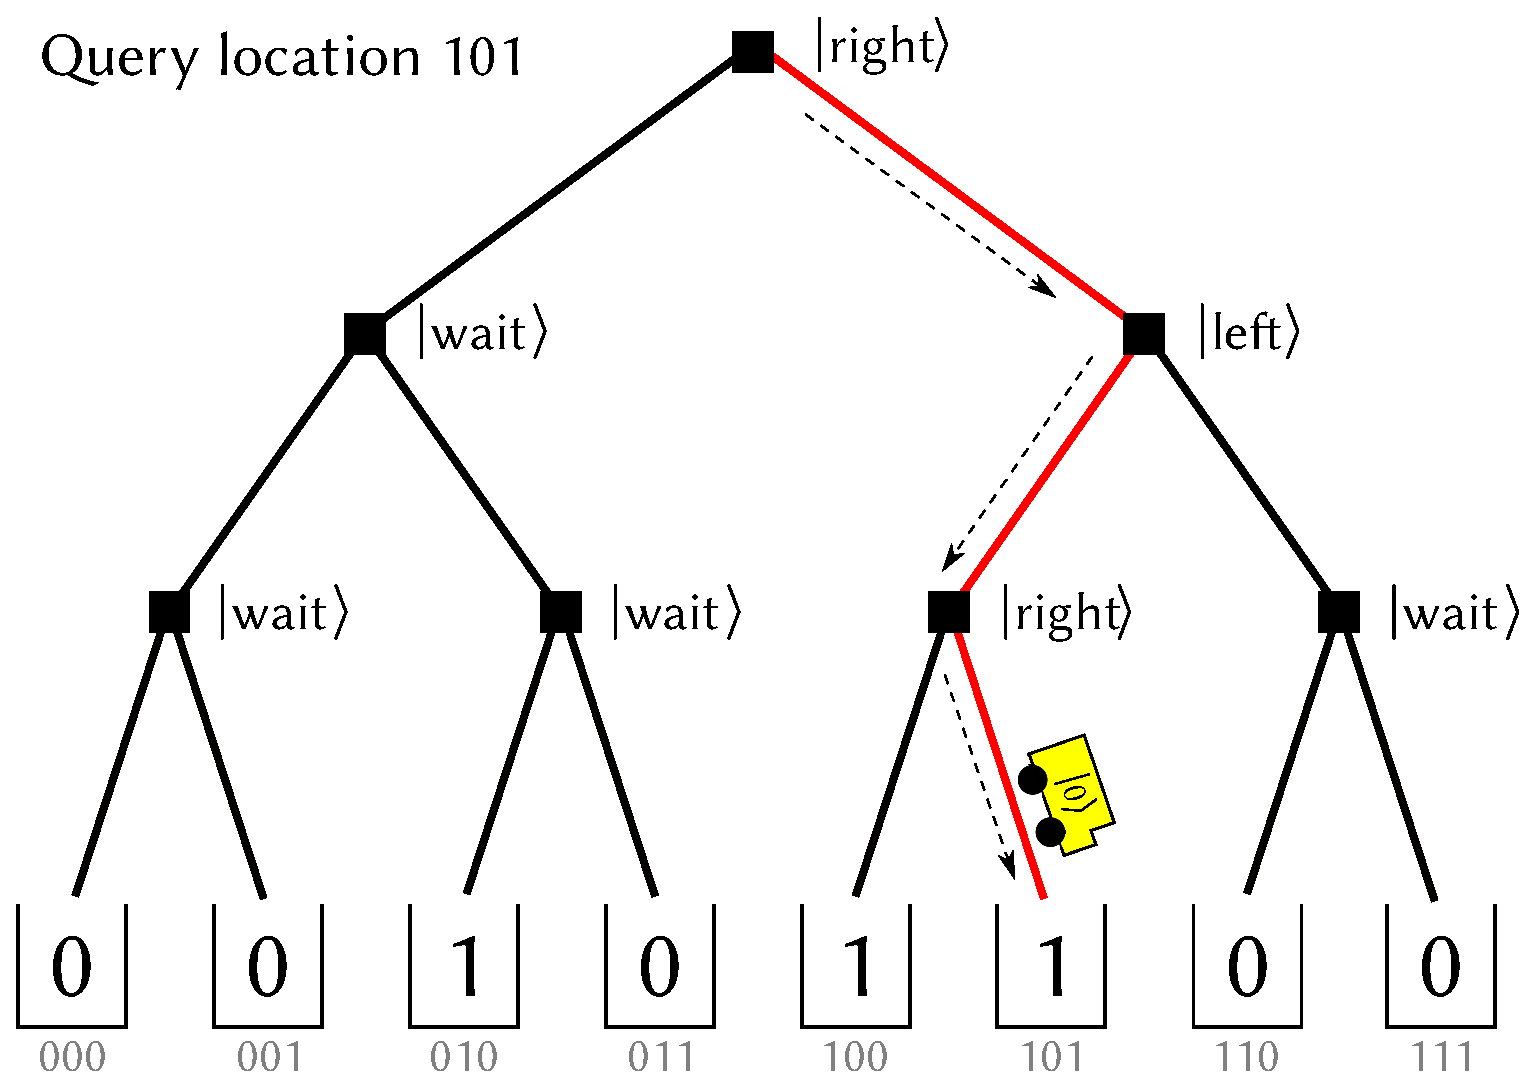
\includegraphics[height=2in]{fig/bb-02}
    \end{subfigure}
    \hspace{0.5cm}
    \begin{subfigure}
        \centering
        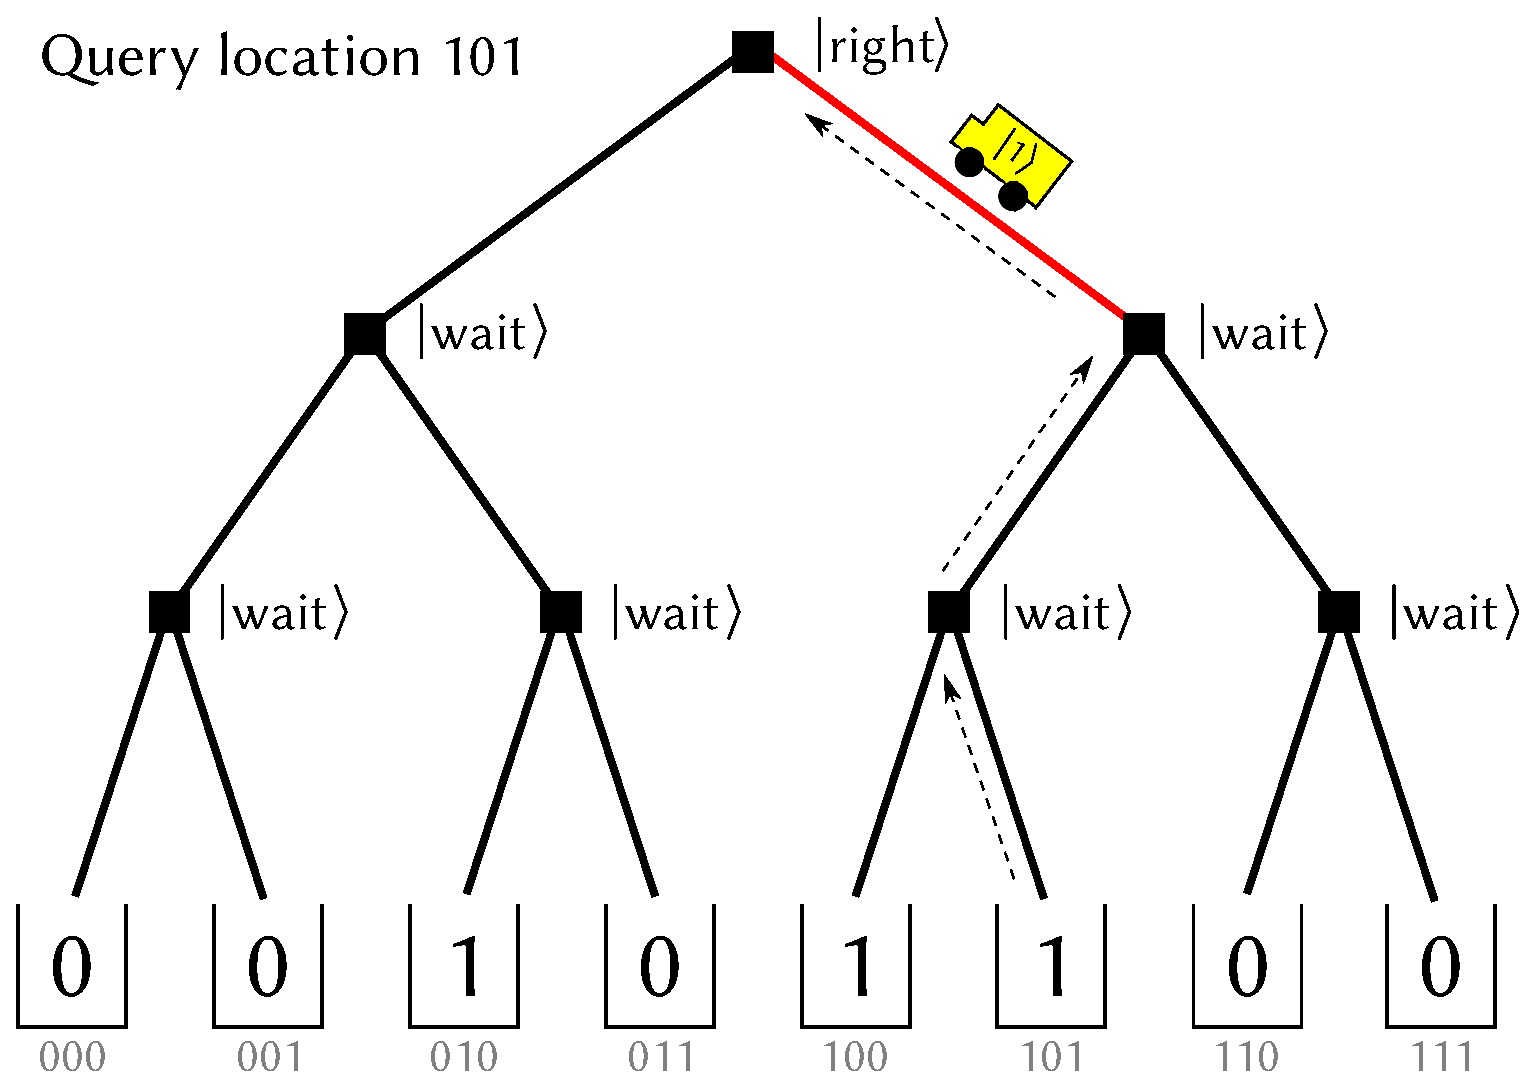
\includegraphics[height=2in]{fig/bb-03}
    \end{subfigure}
    \caption{Schematic of a bucket brigade quantum RAM query. (Top left) Memory contents are stored in the leaves of a binary tree, whose nodes are denoted by qutrits with possible states $\ket{\hbox{wait}}, \ket{\hbox{left}}$, and $\ket{\hbox{right}}$. (Top right) A bucket brigade RAM query is set up by sequentially sending in address qubits to change the qutrit states until a path to the desired cell is created. (Bottom left) To extract the contents of the memory cell, a `bus' photon is used. The photon is directed to the desired cell by the qutrits, where it couples to the memory cell and copies its contents. (Bottom right) The bus photon travels back through the qRAM, resetting the qutrit states to $\ket{\hbox{wait}}$ on its way out.}
\end{figure}


At each node is a three-level state (a qutrit), with levels denoted by $\ket{\hbox{wait}}, \ket{\hbox{left}}, \ket{\hbox{right}}$. All the qutrits begin in $\ket{\hbox{wait}}$. Address qubits are then sent through one by one and the $j$-th bit follows a path to the $j$-th layer. When a qubit reaches a qutrit in its destination layer, it changes the state of that qutrit. An address bit in 0 initiates a unitary operation that sends $\ket{\hbox{wait}} \rightarrow \ket{\hbox{left}}$, while a 1 sends $\ket{\hbox{wait}} \rightarrow \ket{\hbox{right}}$. To reach their destination layers, the qubit simply follows the path directed by the qutrits. After all the address qubits are sent, a quantum `bus' traverses the path, couples to the desired memory cell to gather the data, and is reflected back the way it came. All the nodes are then re-initialized to the $\ket{\hbox{wait}}$ state.


\subsection{How it works}

\subsection{Bit query circuit model}

\subsection{Phase query circuit model}

\subsection{Analysis}


%%%%%%%%%%%%%%%%%%%%%%%%%%%%%%%%%%%%%%%%%%%%%%%%%%%%%%%%%%%%%%%%%%%%%%%%%%%%%%%%%%
%%%%%%%%%%%%%%%%%%%%%%%%%%%%%%%%%%%%%%%%%%%%%%%%%%%%%%%%%%%%%%%%%%%%%%%%%%%%%%%%%%
%%%%%%%%%%%%%%%%%%%%%%%%%%%%%%%%%%%%%%%%%%%%%%%%%%%%%%%%%%%%%%%%%%%%%%%%%%%%%%%%%%
%%%%%%%%%%%%%%%%%%%%%%%%%%%%%%%%%%%%%%%%%%%%%%%%%%%%%%%%%%%%%%%%%%%%%%%%%%%%%%%%%%
%%%%%%%%%%%%%%%%%%%%%%%%%%%%%%%%%%%%%%%%%%%%%%%%%%%%%%%%%%%%%%%%%%%%%%%%%%%%%%%%%%

\section{Quantum ROM}
\label{sec:circuits}

\subsection{Quantum ROM}

\subsection{Efficient state preparation with a qROM}

Discuss \cite{Vadym2018}

\subsection{Optimizing quantum ROMs}

\subsection{Problem-specific qROMs}

Talk about the qROM in \cite{Babbush2018}
%%%%%%%%%%%%%%%%%%%%%%%%%%%%%%%%%%%%%%%%%%%%%%%%%%%%%%%%%%%%%%%%%%%%%%%%%%%%%%%%%%
%%%%%%%%%%%%%%%%%%%%%%%%%%%%%%%%%%%%%%%%%%%%%%%%%%%%%%%%%%%%%%%%%%%%%%%%%%%%%%%%%%
%%%%%%%%%%%%%%%%%%%%%%%%%%%%%%%%%%%%%%%%%%%%%%%%%%%%%%%%%%%%%%%%%%%%%%%%%%%%%%%%%%
%%%%%%%%%%%%%%%%%%%%%%%%%%%%%%%%%%%%%%%%%%%%%%%%%%%%%%%%%%%%%%%%%%%%%%%%%%%%%%%%%%
%%%%%%%%%%%%%%%%%%%%%%%%%%%%%%%%%%%%%%%%%%%%%%%%%%%%%%%%%%%%%%%%%%%%%%%%%%%%%%%%%%

\section{Hardware proposals for qRAM}
\label{sec:hardware}



%%%%%%%%%%%%%%%%%%%%%%%%%%%%%%%%%%%%%%%%%%%%%%%%%%%%%%%%%%%%%%%%%%%%%%%%%%%%%%%%%%
%%%%%%%%%%%%%%%%%%%%%%%%%%%%%%%%%%%%%%%%%%%%%%%%%%%%%%%%%%%%%%%%%%%%%%%%%%%%%%%%%%
%%%%%%%%%%%%%%%%%%%%%%%%%%%%%%%%%%%%%%%%%%%%%%%%%%%%%%%%%%%%%%%%%%%%%%%%%%%%%%%%%%
%%%%%%%%%%%%%%%%%%%%%%%%%%%%%%%%%%%%%%%%%%%%%%%%%%%%%%%%%%%%%%%%%%%%%%%%%%%%%%%%%%
%%%%%%%%%%%%%%%%%%%%%%%%%%%%%%%%%%%%%%%%%%%%%%%%%%%%%%%%%%%%%%%%%%%%%%%%%%%%%%%%%%

\section{Outlook}
\label{sec:outlook}

%%%%%%%%%%%%%%%%%%%%%%%%%%%%%%%%%%%%%%%%%%%%%%%%%%%%%%%%%%%%%%%%%%%%%%%%%%%%%%%%%%
%%%%%%%%%%%%%%%%%%%%%%%%%%%%%%%%%%%%%%%%%%%%%%%%%%%%%%%%%%%%%%%%%%%%%%%%%%%%%%%%%%
%%%%%%%%%%%%%%%%%%%%%%%%%%%%%%%%%%%%%%%%%%%%%%%%%%%%%%%%%%%%%%%%%%%%%%%%%%%%%%%%%%
%%%%%%%%%%%%%%%%%%%%%%%%%%%%%%%%%%%%%%%%%%%%%%%%%%%%%%%%%%%%%%%%%%%%%%%%%%%%%%%%%%
%%%%%%%%%%%%%%%%%%%%%%%%%%%%%%%%%%%%%%%%%%%%%%%%%%%%%%%%%%%%%%%%%%%%%%%%%%%%%%%%%%

\bibliography{primer}
\bibliographystyle{unsrt}

\end{document}
